\chapter{INTRODUCTION}

\section{What is {\LaTeX}}

{\LaTeX} is a document preparation system for high-quality typesetting. It is most often used for medium-to-large technical or scientific documents but it can be used for almost any form of publishing \citep{Carvalho-etal-2008}.  {\LaTeX} is not a word processor! Instead,  {\LaTeX} encourages authors not to worry too much about the appearance of their documents but to concentrate on getting the right content. Let say an author type their work in most typesetting or word-processing systems, he would have to decide what layout to use, for example select:

\begin{itemize}
\item {\Large18pt Times Roman} for the {\Large TITLE}
\item 12pt Times \emph{Italic} for the \emph{NAME}
\item \textbf{bold} for the \textbf{TITLE}
\item Adding or deleting figures or tables
\item Adding or deleting references and formulae
\item and so on...
\end{itemize}

This has two results: authors wasting their time with designs; and a lot of badly designed documents! Especially when it comes to writing a lengthly document such as thesis, books or monograph. {\LaTeX} is based on the idea that it is better to leave document design to document designers, and to let authors get on with writing documents.

In {\LaTeX}:
\begin{itemize}
\item You don't (usually) see the final version of the document when editing it.
\item You generally need to know the necessary commands for LaTeX markup.
\item It can sometimes be difficult to obtain a certain look for the document.
\end{itemize}

On the other hand, there are certain advantages to the {\LaTeX} approach:
\begin{itemize}
\item Document sources can be read with any text editor and understood, unlike the complex binary and XML formats used with WYSIWYG programs.
\item You can concentrate purely on the structure and contents of the document, not get caught up with superficial layout issues.
\item You don't need to manually adjust fonts, text sizes, line heights nor text flow for readability, as {\LaTeX} takes care of them automatically.
\item In {\LaTeX} the document structure is visible to the user, and can be easily copied to another document. In WYSIWYG applications it is often not obvious how a certain formatting was produced, and it might be impossible to copy it directly for use in another document.
\item The layout, fonts, tables and so on are consistent throughout the document.
\item Mathematical formulae can be easily typeset.
\item Indexes, footnotes, citations and references are generated easily.
\item You are forced to structure your documents correctly.
\end{itemize}

{\LaTeX} is based on Donald E. Knuth's {\TeX} typesetting language or certain extensions. {\LaTeX} was first developed in 1985 by Leslie Lamport, and is now being maintained and developed by the \LaTeX3 Project. {\LaTeX}  is available for free by anonymous ftp. The best source for news on {\TeX} and {\LaTeX} is the {\TeX} Users Group. A lot of documentation, and references to even more material, can be found in this documentation section. And in case you were wondering, {\LaTeX} is pronounced Lah-tech or Lay-tech, to rhyme with blech or Bertolt Brecht (almost).

\section{Basic concepts}

An author writes a {\LaTeX} input file in a text editor and then compiles this using {\LaTeX}. An input file contains text and commands for processing the text. There are some conceptual similarities to a markup language such as HTML. However, a fundamental difference is that {\LaTeX} is designed as a page layout language, unlike HMTL which is functional markup. The whole point of {\LaTeX} is to achieve perfect typographic output, which is not the purpose of HTML. {\LaTeX} produces device-independent DVI files,from which you can generate PDF and PostScript files using the utilities that usually come with a {\LaTeX} installation. Typically, you can also create a PDF file directly, as shown in the next section. However, {\LaTeX} is very fussy. A trivial mistake may mean that no output is generated and many error messages are displayed. You will need to check the error logs, fix the problem and recompile. Obtaining more information {\LaTeX} is far more powerful and far more complex than this simple introduction suggests. The Comprehensive TeX Archive Network (CTAN) is the authority for materials that relate to TeX and {\LaTeX} (www.ctan.org).

\section{Working with MiKTex}

MiKTeX is a typesetting system for Microsoft Windows that is developed by Christian Schenk. It consists of an implementation of {\TeX} and a set of related programs. MiKTeX provides the tools necessary to prepare documents using the \TeX/\LaTeX markup language, as well a simple tex editor (TeXworks). MiKTeX can update itself by downloading new versions of previously installed components and packages, and has an easy installation process. Additionally, it can ask users whether they wish to download any packages that have not yet been installed but are requested by the current document. The current version of MiKTeX is 2.9 and is available at the MiKTeX homepage. Since version 2.7, MiKTeX has support for XeTeX, MetaPost and pdfTeX and compatibility with Windows 7.

\subsection{Installation}

Before installing make sure you have a compatible operating systems. MiKTeX 2.8 is compatailbe with the following OS: 

\begin{itemize}
\item Windows 7
\item Windows Server 2008
\item Windows Vista
\item Windows Server 2003
\item Windows XP
\item Windows 2000
\end{itemize}

Please note that MiKTeX 2.8 does not work on legacy Windows platforms (Windows 9x/Me/NT).

\subsubsection{How do I download MiKTeX?}	

It is recommended that you download the “Basic MiKTeX Installer”. This allows you set up a basic MiKTeX system. Download the “MiKTeX Net Installer”, if you want to set up a complete MiKTeX system.

\subsubsection{How do I install MiKTeX?}	

You use one of the installers to set up a a MiKTeX system: Basic MiKTeX Installer (basic-miktex-2.8.xxxx.exe). The “Basic MiKTeX” installer can be used to set up a basic MiKTeX system.

MiKTeX Net Installer (setup-2.8.xxxx.exe). The “MiKTeX Net Installer” can be used to set up a complete MiKTeX system. For more information, read the section Installing MiKTeX in the MiKTeX manual.

\subsubsection{What is the “Basic MiKTeX” installer?}	

The “Basic MiKTeX Installer” sets up a basic MiKTeX system. Additional packages can be installed on-the-fly. This has the advantage of keeping a minimal MiKTeX system.	

\subsubsection{What is the MiKTeX Net Installer?}	

This installer serves two purposes; It downloads all available package archive files to your computer and it installs MiKTeX.

\section{Preamble file}

The source file of a LaTeX broadly consists of two parts, the preamble and the document itself. The preamble is everything from the start of the LaTeX source file until the \verb+\begin{document}+ command. It normally contains commands that affect the entire document. Things like margin settings, document style definitions, paragraph spacing settings, custom function definition and page numeration style are items that are set in the preamble. Often, much of the preamble is placed in a separate file and included using the \verb+\usepackage{subfigure}+ statement. This allows you to use the same code in many source files by just including a single line in each source file.\\

In the \verb+UMP LaTeX User Manual+ folder the preamble file is named \verb+UMP template+. All the codes in the preamble is done to produce your thesis according to the UMP format. To have a consistent result do not change the preamble code except in the \verb+\mainmatter+ section.  

\subsection{Installing userpackage}

Add-on features for {\LaTeX} are known as packages. Dozens of these are pre-installed with {\LaTeX} and can be used in your documents immediately. They should all be stored in subdirectories of texmf/tex/latex named after each package. To find out what other packages are available and what they do, you should use the CTAN search page which includes a link to Graham Williams' comprehensive package catalogue.\\ 

A package is a file or collection of files containing extra LaTeX commands and programming which add new styling features or modify those already existing. Installed package files all end with .sty (there may be ancillary files as well). When you try to typeset a document which requires a package which is not installed on your system, {\LaTeX} will warn you with an error message that it is missing, and you can then download the package and install it using the instructions in the installing extra packages section. You can also download updates to packages you already have (both the ones that were installed along with your version of {\LaTeX} as well as ones you added). If your are using MiKTeX and {\LaTeX} gives you a warning that some userpackage is missing you can download it using Package Manager (Figure \ref{fig2:package_manager}).

\begin{figure}
	\centering
	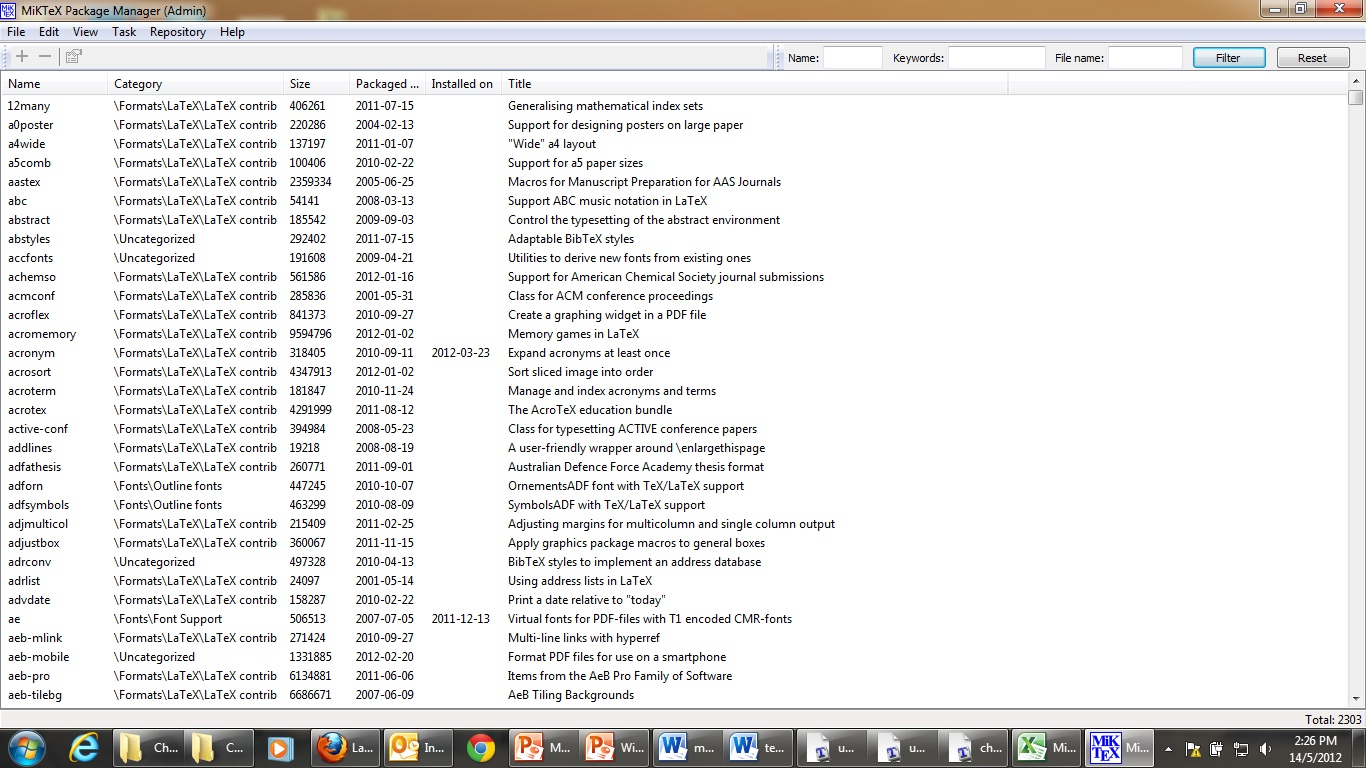
\includegraphics[width=1.00\textwidth]{admin_package} 
	\caption{Package Manager GUI}
	\label{fig2:package_manager}
\end{figure}

\section{Document file}

Using any text editor you can make a document file. Such raw text is referred to as {\LaTeX} source. Using the LaTeX program, it is converted to a beautifully formatted document. The content of the document is typed as plain text into one or more \verb+.tex+ files. Raw bibliographic databases are in plain text files named with the suffix \verb+.bib+ which we name it as \verb+rujukan_ump+.\\

In this work, the user only need to create different \verb+.tex+ file for each chapter and the file is located in a separate folder. For example, \verb+chap1.tex+ is located in the \verb+Chap1+ folder while \verb+chap2.tex+ is located in \verb+Chap2+ folder and so on. Note that in the preamble file, in the \verb+\mainmatter+ section only two chapters are included. If you have more just add \verb+\chapter{METHODOLOGY}
\label{ch:tocloft}

\section{Parametric Representation of curves and surfaces}


[1] Rogers. David F., An introduction to NURBS with historical perspective. 2001 by Academic Press.


The standard for describing and modeling curves and surfaces in computer aided design (CAD) and computer graphics is NURBS, or NonUniform Rational B-Splines. Essentially, NURBS describe parametric curves and surfaces. Curves and surfaces are mathematically represented either explicitly, implicitly or parametrically.

In practice, curves and surfaces are generally bounded. When either an explicit or implicit representation is used, imposing the boundaries is awkward. In contrast, the boundaries for a parametrically represented curve or surface are provided by the restective parameter ranges. In addition, the parameter range for a parametric curve also specifies a natural traversal direction along the curve. For example, specifying a curve requires one parameter while specifying a surface requires 2 parameters.

In general, a parametric curve representation of a 3D curve takes the mathematical functional form of x=f(t), y=g)t), and z=h(t), where t is the independent parameter. By extension, a parametric surface representation takes the form of x=f(u,w), y=g(u,w), z=h(u,w), where u and w are independent parameters. When compared to either explicit or implicit formulations, this parametric representation is extremely flexible. The representation is axis independent, easily represented by multiple-valued functions, can have infinite derivatives, and extended degrees of freedom.  To have more degrees of freedom additional independent parameters can be added.

\section{Continuity of curves and surfaces}

There are two kinds of continuity, or smoothness, associated with parametric curves and surfaces known as geometric continuity and parametric continuity. Simplistically, you can think of geometric continuity as physical and parametric continuity as mathematical. Geometric continuity is less restrictive than parametric continuity.




\section{Advantages of Parametric Representations in CNC}



\section{Parametric representation to CNC G-Codes}






All auto-numbered headings get entered in the Table of Contents (ToC) automatically. Entries for the ToC are recorded each time you process your document, and reproduced the next time you process it, so you need to re-run {\LaTeX} one extra time to ensure that all ToC page number references are correctly calculated. The commands \verb+\listoffigures+ and \verb+\listoftables+ work in exactly the same way as \verb+\tableofcontents+ to automatically list all your tables and figures. Note that, to have your figures or tables listed in list of figures or tables the command \verb+\ref{}+ must be used for referring the designated figure or table. Details on this will be given the following chapters.\\

The primary way to build a table is to use the tabular environment. Here's an example:

\begin{tabular}[t]{|l|ccccc|c|}
\multicolumn{7}{c}{USAMTS Scores Round 1}\\\hline
Name&\#1&\#2&\#3&\#4&\#5&Total\\\hline
John Doe&5&5&3&2&1&16\\
Jane Doe&5&5&5&4&5&24\\
Richard Feynman&5&5&5&5&5&25\\\hline
\end{tabular}

When you typeset that code, you should see a simple table like this one. Read through the following general description of the tabular environment to understand how the code above produced the table.\\

General form of the tabular environment:
\verb+\begin{tabular}[alignment]{columns}+
\verb+rows+
\verb+\end{tabular}+\\

\textbf{alignment} - put either b or t, or omit this completely. This determines how your table is vertically positioned with the text around it. This entry is not too important - experiment using different values (or omitting it) when you have a table in the midst of a document to get a better feel for it.\\

\textbf{columns} - this describes the number of columns and the alignment of each column. Put r for a right-justified column, c for a centered column, and l for a left-justified column. Put a | if you want a vertical line between columns. For example, the column declaration \verb+{||rr|cc|l}+ will produce a table that has 2 vertical lines on the left, then two columns that are right-justified, then a vertical line, then 2 columns that are centered, then another vertical line, then a left-justified column. There are more complicating things that you can do, and even more complicated things if you include the array packing in your document (check a good LaTeX book for more details), but for most tables, the options we've described here are sufficient.\\

\textbf{rows} - You can have as many rows as you like. For each row, you need an entry for each column. Each of these entries is separated by an \verb+&+. Use \verb+\\+ to indicate that your input for that row is finished. Hence, if your column declaration was \verb+{cccc}+, a possible row entry could be \verb+5&5&5&5\\+
\\

If you wish for one row to have fewer columns (i.e. one column takes up several of the usual table columns), use the command \verb+\multicolumn+. In the example above, we had as our first row\\

\verb+\multicolumn{7}{c}{USAMTS Scores Round 1}\\+

The first \verb+{ }+ indicates how many regular columns this entry will take up. The second \verb+{ }+ indicates whether the text in this entry is right (r), left (l) or center (c) justified. The final \verb+{ }+ contains our entry. As with the regular column declaration, use | if you want a vertical line before or after the entry of \verb+\multicolumn+.\\

In general, you can use \verb+\vline+ to introduce a vertical line anywhere in a table (try putting one between John and Nash in the example below and see what happens).\\

Finally, at the end of some of the rows in our example, we have the command \verb+\hline+. This produces a horizontal line after the row it follows. If you want a horizontal line atop a table, use \verb+\hline+ right before the first row. If you only want a horizontal line under a portion of the row, use \verb+\cline{start column-end column}+ as indicated in the example below:\\

\begin{tabular}[t]{|l|l|cccc|c|}\hline
\multicolumn{7}{|c|}{USAMTS Final Scores by Round}\\\hline
Medal&Name&\#1&\#2&\#3&\#4&Total\\\hline\hline
&Richard Feynman&25&25&25&25&100\\\cline{3-7}
Gold&Albert Einstein&25&25&25&25&100\\\cline{3-7}
&Marie Curie&25&24&24&25&98\\\hline
Silver&John Nash&20&20&25&24&89\\\hline
&Jane Doe&23&\multicolumn{2}{c}{None}&25&48\\\cline{3-7}
None&John Doe&\multicolumn{2}{c}{None}&25&20&45\\\cline{3-7}
&Lazy Person&5&\multicolumn{3}{c|}{None}&5\\\hline
\end{tabular}

When you typeset this, you should get output like this. Note how we made a double horizontal line after the table headings.\\

Finally, sometimes you'll want to create a table that consists solely of items in math mode. For such a table, use the array environment. The array environment works exactly like tabular, except that all its entries are rendered in math mode:

\[\begin{array}[b]{ccc}
x&y&z\\
y&x&z\\
1&2&3
\end{array}\]

Change both array declarations to tabular and delete the \verb+\[+ and \verb+\]+ and see what happens. You can do a number of other things with the array and tabular environments, but the above should cover most of what you'll want to do with them.\\

If you build a table in which some entries are text that will take up multiple lines, you'll probably want to learn about boxes (below).

+ to the list. Make sure you have created the designated folder and file for that chapter. \\

To keep thing simple so that user can directly use the application, open the \verb+chap1.tex+ in \verb+Chap1+ folder. Initially you will have a blank document. This document will contain all your writing for a chapter. For subsequent chapter create another document file. An example of completed document file is shown in Figure \ref{fig1:example_file}.

\begin{figure}
	\centering
	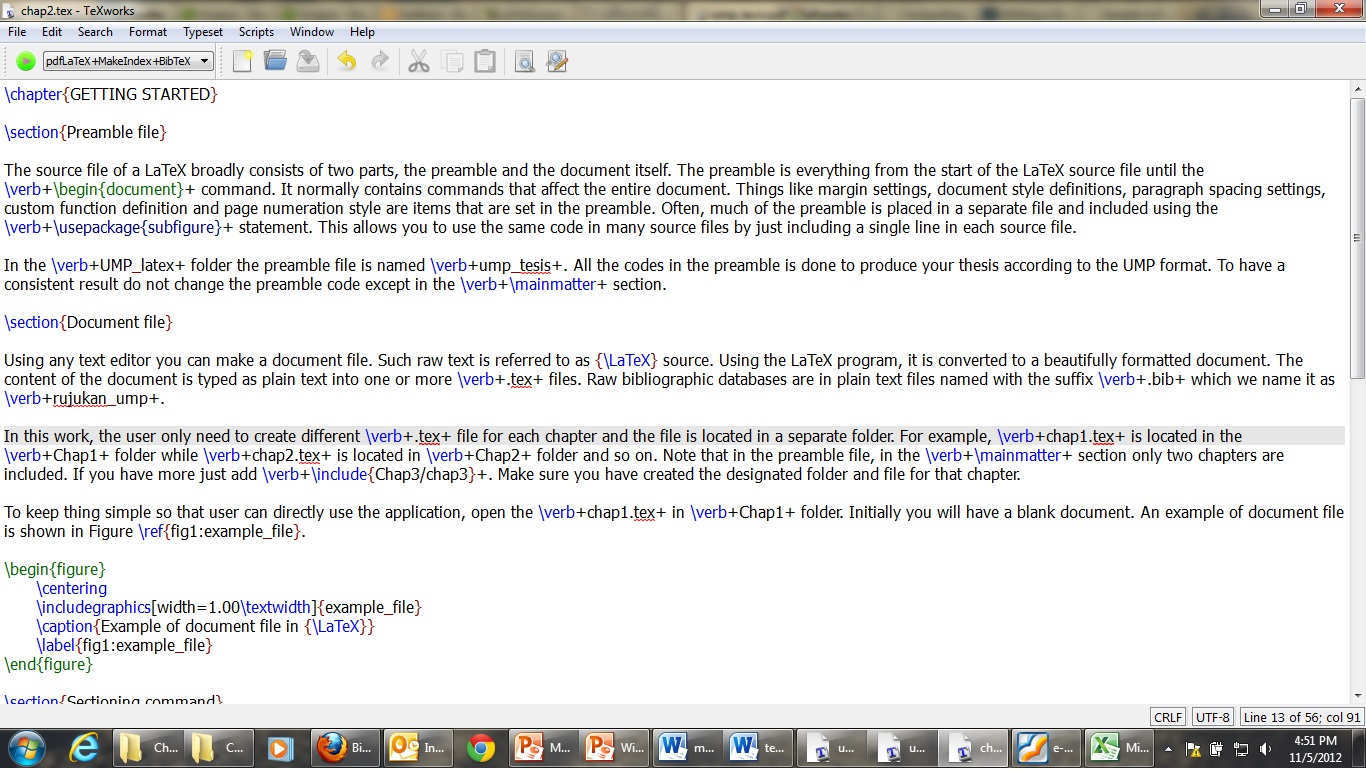
\includegraphics[width=1.00\textwidth]{example_file} 
	\caption{Example of document file in {\LaTeX}}
	\label{fig1:example_file}
\end{figure}

\section{Typesetting your file and viewing output pdf file}
Once you are ready to take a look at how your document will appear you typeset it with the default engine, pdflatex out of the box, by simply using the \verb+Typeset+ command.\\

Assuming the document was successfully typeset the pdf file will automatically open in a separate preview window.







